\documentclass[../reportesINE.tex]{subfiles}

\begin{document}

\subsection{Arquitectura de servidores}
Los entornos de contenido web que se necesitan para el sistema y los servidores necesarios para cada entorno se muestran en la \textit{Imagen \ref{fig:arquitectura}}. Esta información permite asegurarse de que se tienen todos los recursos de hardware necesarios para dar soporte al sitio de contenido web. \\ \\
El equipo de arquitectura técnica también documenta una arquitectura de servidor para cada servidor descrito en la arquitectura de entorno. Una arquitectura de servidor describe la configuración detallada de cada servidor e incluye: \\ 
\begin{itemize}
\item Hardware que se necesita para cada servidor
\item Sistema operativo que se necesita para cada servidor
\item Software que se necesita
\item Valores de configuración para todo el hardware, software y sistemas operativos
\item tras relaciones como, por ejemplo, las de repositorios de datos remotos y repositorios de usuarios \\
\end{itemize} 

Por la modularidad que se tiene en el sistema, se acordó que el módulo de consulta tuviera su propio WAR\footnote{Un archivo WAR (de Web Application Archive - Archivo de aplicación web) es un archivo JAR utilizado para distribuir una colección de JavaServer Pages, servlets, clases Java, archivos XML, bibliotecas de tags y páginas web estáticas (HTML y archivos relacionados) que juntos constituyen una aplicación web.} para desarrollo.

\begin{figure}[h]
  \centering
  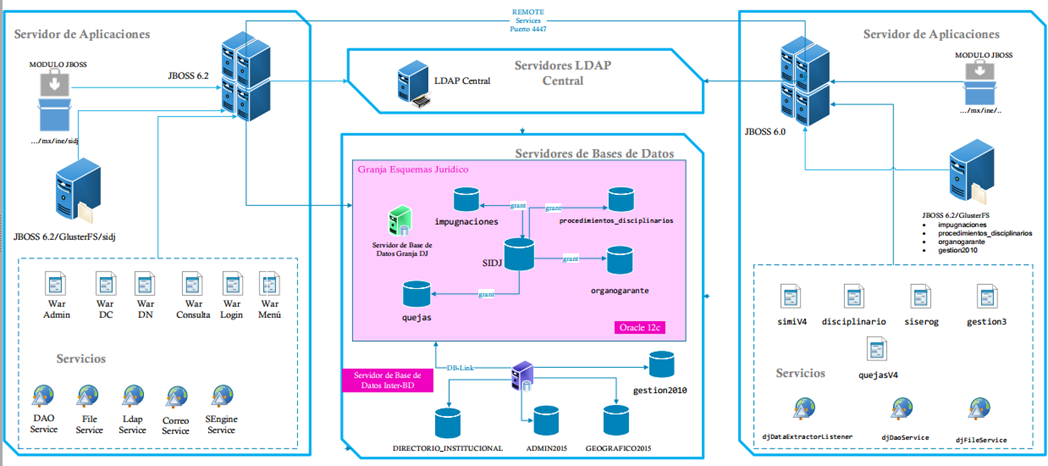
\includegraphics[width=\linewidth]{img/arquitectura.png}
  \caption{Arquitectura de servidores del Sistemas de la Dirección Jurídica.}
  \label{fig:arquitectura}
\end{figure}


\subsection{Esquema general de software}
Debido a la alta demanda de peticiones que pueden llegar al sistema el esquema de servidores se dividió en cuatro categorías: servicios WEB, aplicaciones, LDAP y Base de Datos.  \\ \\
De este modo se logra distribuir y balancear la carga de trabajo evitando que los servidores se saturen consiguiendo que el tiempo de respuesta y el desempeño del sistema sean eficientes. \textit{Imagen \ref{fig:esquemaGeneral}}

\begin{figure}[h]
  \centering
  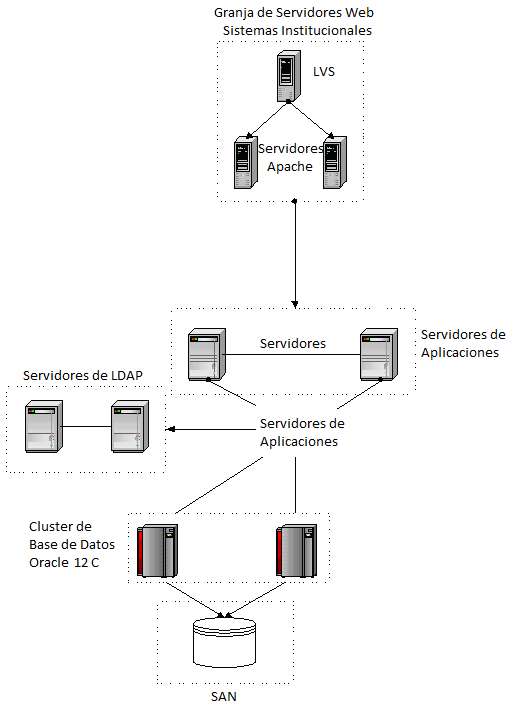
\includegraphics[width=\linewidth]{img/esquemaGeneral.png}
  \caption{Esquema general del Sistemas de la Dirección Jurídica.}
  \label{fig:esquemaGeneral}
\end{figure}

\subsection{Módulos del sistema}
En la \textit{Imagen \ref{fig:organizacionModulos}} se muestra la organización de módulos disponibles en el \textit{Sistema Integral de la Dirección Jurídica}, en este reporte nos enfocamos en el módulo de consulta. Se muestran también los sub-módulos correspondientes. 

\begin{figure}[h]
  \centering
  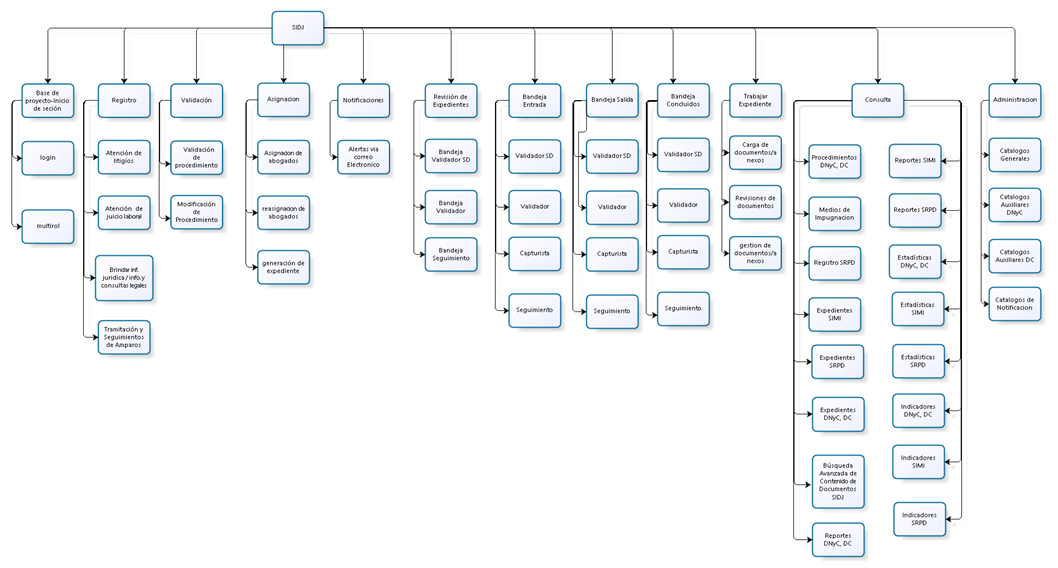
\includegraphics[width=\linewidth]{img/organizacionModulos.png}
  \caption{Organización de módulos en el Sistemas de la Dirección Jurídica.}
  \label{fig:organizacionModulos}
\end{figure}
\clearpage

\subsection{Arquitectura de software}
La Arquitectura del Software es el diseño de más alto nivel de la estructura de un sistema. Es un conjunto de patrones y abstracciones coherentes que proporcionan un marco definido y claro para interactuar con el código fuente de la aplicación. \\ \\
El \textit{Sistema Integral de la Dirección Jurídica} es una aplicación desarrollada en Spring, definida en jerarquías de tipos (clases o interfaces) construidas en capas, a continuación explico brevemente cada una de ellas. 
Comenzaré “de abajo a arriba”, es decir, partiré definiendo las entidades persistentes con Hibernate, e iré “subiendo” hasta la capa de presentación y control con JSF, pasando antes por el negocio (el modelo) con Spring.

\subsubsection{La capa de persistencia}
En esta capa están ubicadas las entidades de la aplicación, mapeadas a clases con Hibernate. \\ \\
Se llama “persistencia” de los objetos a su capacidad para guardarse y recuperarse desde un medio de almacenamiento. La persistencia en Base de Datos relacionales se suele implementar mediante el desarrollo de funcionalidad específica utilizando la tecnología JDBC o mediante frameworks que automatizan el proceso a partir de mapeos (conocidos como Object Relational Mapping, ORM) como es el caso de Hibernate.

\subsubsection{El DAO}
El DAO es el Data Access Object, es decir, será la clase donde resida la lógica de manejo de Hibernate. De esta forma conseguimos que nuestra lógica de negocio no sepa nada de Hibernate, y siempre que quiera acceder a los datos lo hara usando esta clase. \\ \\
Este patrón de diseño divide más las responsabilidades en la aplicación de tal forma que tendremos unas clases que se encargaran de la lógica de negocio y otras clases la responsabilidad de persistencia.

\subsubsection{La capa de negocio}
Lo único que hace es delegar en el DAO, hay quien me podría acusar de estar cayendo en el antipatrón “Poltergeist”, ya que desde control podríamos usar directamente el DAO para recuperar o guardar los productos, y quitarnos esta clase de enmedio. Pero no creo que este sea el caso ya que prima el MVC y el bajo acoplamiento. \\
Siempre debemos intentar que la capa de control y presentación sean lo más tontas posibles. Pensar por un momento que no usamos esta clase “manager” y que usamos el DAO desde las clases de control de JSF (los managed-beans). 

\subsubsection{La capa de control}
En esta capa todas las peticiones realizadas por el usuario son procesadas y distribuidas a la capa de negocio correspondiente. También esta encargada de la interacción que pueda tener un módulo. 

\subsubsection{La capa de presentación}
Aquí se encuentra la vista del sistema con la que el usuario va a interactuar. Todos los componentes del sistema como botones, campos de texto, menús, ligas de acceso, etc están declarados en esta capa.


\subsection{Vista lógica para el módulo de consulta}
La arquitectura definida para la implentación de los módulos correspondientes al sistema es mostrada en el diagrama de la \textit{Imagen \ref{fig:asoftgeneral}}.

\begin{figure}[h]
  \centering
  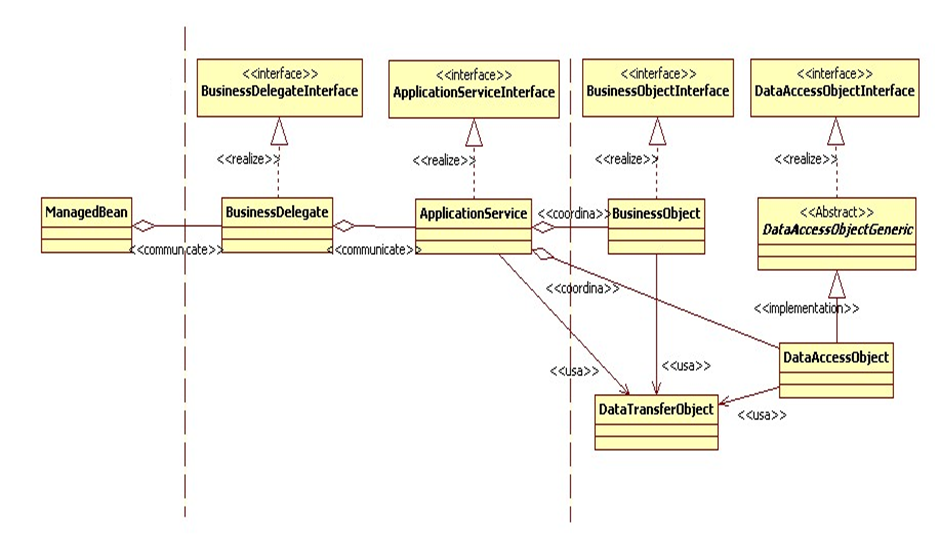
\includegraphics[width=\linewidth]{img/asoftgeneral.png}
  \caption{Arquitectura de implementación para el Sistemas de la Dirección Jurídica.}
  \label{fig:asoftgeneral}
\end{figure}

Tomando en cuenta la arquitectura establecida en el desarrollo,  el diagrama de la \textit{Imagen \ref{fig:asoftmodulo}}  muestra una descripción general de la implementación del módulo de consulta, tomando en cuenta las capas planteadas para el desarrollo.

\begin{figure}[h]
  \centering
  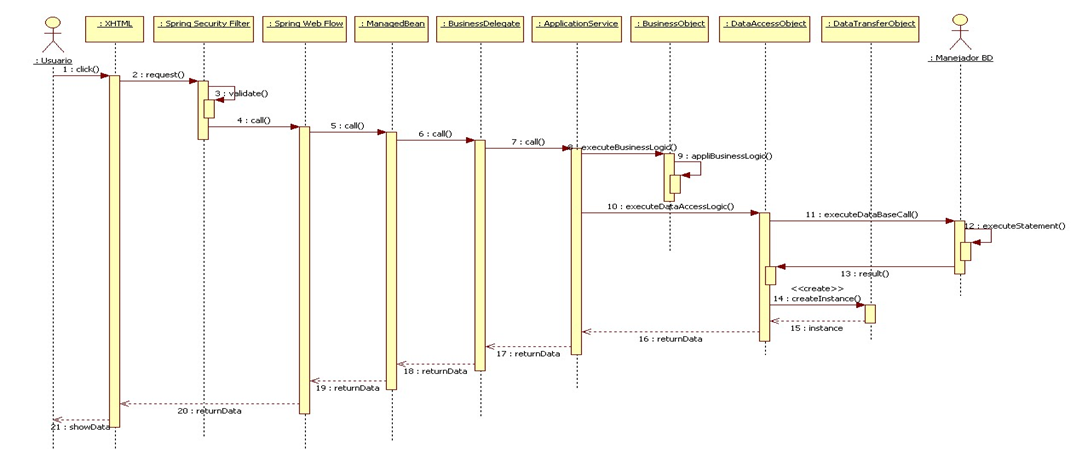
\includegraphics[width=\linewidth]{img/asoftmodulo.png}
  \caption{Arquitectura de implementación para el módulo de reportes.}
  \label{fig:asoftmodulo}
\end{figure}

\subsection{Tecnologías, frameworks y software de \\ desarrollo}
\begin{tabular}{ c c c }
 \textbf{Nombre} & \textbf{Uso} & \textbf{Versión} \\ 
 Java SE & Lenguaje de Desarrollo & 7.0 \\  
 Jboss EAP & Servidor de aplicaciones & 6.2 \\
 JSF & Vista de la aplicación & 4.0.3 \\
 PrimeFaces-EXT & Componentes adicionales para PrimeFaces & 1.1.0 \\
 Simple-captcha & Captcha de la aplicación & 1.2.1 \\
 Spring-security & Login, control de acceso & 3.1.3 \\
 Spring web flow & Implementación MVC & 2.3.2 \\
 Spring persistence & Persistencia JPA & 3.1.4 \\
 Spring beans & Inyección de dependencia & 3.1.4 \\
 Spring tx & Manejo de transacciones & 3.1.4 \\
 Hibernate 4 & Implementación ORM & 4.0 \\
 iReports & Generación de PDF & 4.7.1 \\
 POI Apache & Manipulación de documentos Microsoft & 3.10
\end{tabular}

\end{document}